\[
\begin{tikzcd}[column sep = huge]
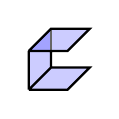
\begin{tikzpicture}[x = 1.4em, y = 1.4em, z = 0.8em, baseline = 0.4em]
    \begin{scope}[fill=blue, opacity=0.2]
    \fill
    (0,0,0) -- (0,1,0) -- (0,1,1) -- (0,0,1) -- (0,0,0);
    \fill
    (0,0,0) -- (1,0,0) -- (1,0,1) -- (0,0,1) -- (0,0,0);
    \fill
    (0,1,0) -- (1,1,0) -- (1,1,1) -- (0,1,1) -- (0,1,0);
    \end{scope}
    \begin{scope}[thick]
    \draw[black!60]
    (0,0.4,1) -- (0,1,1);
    \draw
    (0,0,1) -- (0,0.45,1)
    (0,0,0) -- (0,1,0)
    (0,0,0) -- (1,0,0) -- (1,0,1) -- (0,0,1) -- (0,0,0)
    (0,1,0) -- (1,1,0) -- (1,1,1) -- (0,1,1) -- (0,1,0);
    \end{scope}
\end{tikzpicture}
\ar[r, "\alpha_1\cup c_x\cup\alpha_2"] \ar[d] & E \ar[d, " p"]\\
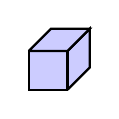
\begin{tikzpicture}[x = 1.4em, y = 1.4em, z = 0.8em, baseline = 0.4em]
    \begin{scope}[fill=blue!20, thick]
    \filldraw
    (1,0,0) -- (1,1,0) -- (1,1,1) -- (1,0,1) -- (1,0,0);
    \filldraw
    (1,0,0) -- (1,1,0) -- (0,1,0) -- (0,0,0) -- (1,0,0);
    \filldraw
    (0,1,0) -- (1,1,0) -- (1,1,1) -- (0,1,1) -- (0,1,0);
    \end{scope}
\end{tikzpicture}
\ar[r, "H"'] \ar[ur, dashed] & B
\end{tikzcd}\rightnote{Note that for this to work we have to \enquote{swap} the last two coordinates!}
\]